\documentclass[12pt]{article}
\usepackage{hyperref}
\usepackage{amsmath, amssymb, amsfonts}
\usepackage[margin=1.5cm]{geometry}
\usepackage{xcolor}
\usepackage{graphicx}
\usepackage{xparse}
\usepackage{enumitem, inconsolata}
\parindent 0px
\newcommand{\lb}{\\$\left|\rightarrow\right.$}
\newcommand{\ra}{\rightarrow}
\newcommand{\enter}{\\\textcolor{white}{1}}
\newcommand{\tab}{\textcolor{white}{11}}
\newcommand{\sub}[1]{\textsubscript{#1}}
\newcommand{\super}[1]{\textsuperscript{#1}}

\ExplSyntaxOn

\NewDocumentCommand{\bo}{m}
 {
   \bold_commas:n { #1 }
 }

\cs_new:Npn \bold_commas:n #1
 {
   \seq_set_split:Nnn \l_tmpa_seq { , } { #1 }
   \seq_map_indexed_function:NN \l_tmpa_seq \__bold_commas_aux:nn
 }

\cs_new:Npn \__bold_commas_aux:nn #1 #2
 {
   \textbf{#2}
   \int_compare:nNnTF { #1 } < { \seq_count:N \l_tmpa_seq }
     { , }
     { }
 }

\ExplSyntaxOff

\title{DBMS}
\author{Me lol\\Bhushan Nepal}
\date{\today}

\begin{document}
\maketitle
\vspace{8cm}
\begin{large}\textbf{Notes}\end{large}
\begin{itemize}
\item PYQs of BEI's CT610, BCT's CT652 are combined.
\item PYQs of BEI's CT610's are styled as \texttt{this font in order to say that these are our syllabus' pyq's}.
\item PYQ of BCT with no subject code mentioned in the question paper, starting from 2068 Magh and earlier, will be \textit{stylized as italic to differentiate them}
\item Months are marked as: 
\begin{itemize}[noitemsep]
	\item Ba: Baisakh
	\item Jth: Jestha
	\item Asa: Ashar
	\item Shr: Shrawan
	\item Bh: Bhadra
	\item Ash: Ashwin
	\item Ka: Kartik
	\item Mng: Mangsir
	\item Po: Poush
	\item Ma: Magh
	\item Ch: Chaitra
\end{itemize}
\end{itemize}

\pagebreak
\tableofcontents
\pagebreak

\section{Introduction}
    \begin{center}(3 Hours/4 Marks)\end{center}
    \subsection{Concepts and Applications}
    \begin{enumerate}
        \item Define data\hfill[1.5] (\bo{\texttt{81 Bh}}) [0.5] (\bo{\texttt{80 Bh}, 79 Ch})
        \item Define DBMS\hfill[1.5] (\bo{\texttt{81 Bh}}) [1] (\texttt{81 Ba}) [0.5] (\bo{\texttt{80 Bh}, 79 Ch})
        \item Distinguish between a database and a DBMS.\hfill [2] (71 Ma)
        \item Mention the advantages of DBMS over file processing system, explain briefly.
        \enter\hfill[3] (\bo{79 Ch}) [4] (\bo{74 Bh})
            \lb What difficulties would you face if you used file system directly to implement a database application?\hfill[3] (\bo{71 Bh})
            \lb Drawbacks of file system.\hfill [4] (72 Ma) [6] (\bo{68 Bh})
            \lb Disadvantages of conventional file system?\hfill[2] (76 Ba)
            \lb What are the advantages of DBMS?\hfill[3] (\texttt{\bo{79 Bh}})
        \item Briefly highlight differences between file-processing system and a DBMS.
        \enter\hfill[2] (\bo{\texttt{80 Bh}}) [4] (\bo{76 Bh, 69 Bh})
        \lb Specifically asked to list and explain 5.\hfill [5] (\bo{67 Mng})
        \item Explain the advantages of using Relational DBMS.\hfill[4] (\bo{80 Ch})
        \item Explain four components of DBMS.\hfill[4] (81 Ba)
        \item List roles and responsibilities of Database Administrator.\hfill[2] (\bo{\texttt{79 Bh}})
        \end{enumerate}
        \subsection{Objective and Evolution}
        \begin{enumerate}
        \item What are the latest trends in Database Management?\hfill[2] (\bo{\texttt{81 Bh}})
        \end{enumerate}

    \subsection{Data Abstraction and Data Independence}
    \begin{enumerate}
    \item Define the terms Data Abstraction and Data Independence.\hfill[2] (\bo{78 Ch})
    \item Define Data Abstraction. \hfill[1] (75 Ba, 73 Ma)
    \item Define data independence and explain its significance.\hfill[2] (76 Ba)
    \item Why are abstraction and independence important in DBMS?\hfill[3] (\bo{78 Ch})
    \item Mention the different levels of data abstraction and explain.\hfill[2] (\bo{75 Bh}) [4] (\bo{70 Bh}, 68 Ma)
    \item Explain data abstraction different levels with suitable example.
    \enter\hfill[2] (\bo{80 Ch, 77 Ch}) [3] (75 Ba, 73 Ma) [4] (70 Bh)
    \item Why is data independence important in data modeling?\hfill[2] (\bo{73 Bh, 72 Ash})
    \item Differentiate between physical and logical data independence.\hfill[2] (\texttt{80 Ba, 72 Ash})
    \item What is physical data independence?\hfill[1] (\bo{71 Bh})
    \item Why is physical data independence important in data modeling?\hfill[2] (\bo{77 Ch})
    \item What is the advantage of separating the logical and physical level in database design?\hfill[2] (71 Ma)
    \item List and explain all the aspects of database system that might be subjects to change in physical storage.\hfill[6] (65 Ka)
    \end{enumerate}

    \subsection{Schema and Instances}
    \begin{enumerate}
    \item What do you mean by scheme and instances?\hfill[2] (\bo{75 Bh}, \texttt{81 Ba})
    \item Differentiate between schema and instances.\hfill[2] (\bo{73 Bh}, 76 Ba)
    \item Explain three schema architecture in DBMS.\hfill[2] (81 Ba)
    \lb (Assumed) Explain z-tier architecture in DBMS.\hfill[2] (\bo{\texttt{80 Bh}})
    (Author's note: \textit{This would make perfect sense if it was 3-tier, but original had z-tier})
    \end{enumerate}
    
    \subsection{Concepts of DDL, DML and DCL}
    \begin{enumerate}
    \item Define DDL, DML, DCL with examples.\hfill[3] (\texttt{80 Ba})
    \item Explain the difference between DDL, DML and DCL along with examples.\hfill[4] (70 Ma)
    \item What is data definition language?\hfill[1] (\bo{\textit{67 Mng}})
    \end{enumerate}

    \pagebreak
\section{Data Models}
    \begin{center}(7 Hours/12 Marks)\end{center}
    \begin{enumerate}
    \item What are data models? Explain various types of data models.\hfill[1+3] (73 Ma)

    \item Explain the relational model of database system along with foreign key constraint with appropriate example.\hfill[4] (\bo{79 Ch})

    \item Explain how network data model is different from relation data model.\hfill[4] (72 Ma)
    \end{enumerate}
    \subsection{Logical, Physical and Conceptual}
    \subsection{E-R Model}
    \begin{enumerate}
    \item Define unary relationship along with example.\hfill[2] (\bo{75 Bh})

    \item How do you convert an ER relationship into relation schema? Explain with examples of different cardinalities.\hfill[4] (\bo{75 Bh})

    \item Describe what is total participation using an ERD example.\hfill[4] (70 Ma)

    \item Differentiate total and partial participation with suitable example.\hfill[4] (\bo{73 Bh})

    \item What is importance of aggregation in ER design? Discuss with an example.\hfill[2] (76 Ba)

    \item Define generalization and specialization with its notation and examples.\hfill[4] (\bo{80 Ch}, 71 Ma)

    \item Mention the distinctions among the terms Generalization and Specification with appropriate symbolic representation.\hspace{11.9cm}[4] (\bo{76 Bh})

    \end{enumerate}
    \subsection{Entities and Entities sets}
    \begin{enumerate}
    \item Explain strong and weak entity sets along with example.\hfill[4] (\bo{\textit{67 Mng}}, 75 Ba)
    \end{enumerate}
    \subsection{Strong and Weak Entity Sets}
    \begin{enumerate}
    \item What is the difference between strong and weak entity sets?\hfill[4] (\bo{72 Ash, 70 Bh})
    \end{enumerate}
    \subsection{Attribute and Keys}
    \begin{enumerate}
    \item Define Attributes and explain its type with example.\hfill[4] (\bo{\texttt{80 Bh}})

    \item Define attribute and its types, entity, participation constraint, weak entity set.\hfill [3] (\texttt{81 Ba})

    \item How do you represent composite and multivalued attributes of ERD in tables? Explain with example.\hfill[4] (\textit{65 Ka})

    \item What is keys and explain different types of keys.\hfill[2] (\texttt{80 Ba})

    \item Explain different keys used in database design.\hfill[2] (\bo{74 Bh})

    \item What is key attribute? List out the types and explain them briefly.\hfill[3] (\bo{\texttt{79 Bh}})
    \end{enumerate}
    \subsection{E-R Diagram}
    \begin{enumerate}
    \item Differentiate between degree with the cardinality of a relationship in an ER diagram.
    \enter\hfill[2] (\bo{\texttt{81 Bh}, 77 Ch}) [4] (\bo{71 Bh, 69 Bh})

    \item Explain briefly about generalization in context to ER diagram with an example.
    \enter\hfill[2] (\bo{\texttt{81 Bh}, 77 Ch})

    \item Define discriminator in ER diagram.\hfill[2] (\bo{74 Bh})

    \item A General Hospital consists of a number of specialized wards (such as Radiology, Oncology, etc). Information about ward includes unique name, total numbers of current patients. Each ward hosts a number of patients, who were admitted by a consultant (doctors) employed by the Hospital. On admission, the date and time are kept. The personal details of every patient include name, Medical Record Number (MRN), set of phone number and one address (city, street, code). A separate register is to be held to store the information of the tests undertaken. Each test has unique episode number, category and the final result of test. Number of tests may be conducted for each patient. Doctors are specialists in a specific ward and may be leading consultants for a number of patient. Each patient is assigned to one leading consultant but may be examined by other doctors, if required. Drawn an ER diagram for the above case implementing necessary design constraints.\hfill[8] (\bo{\texttt{81 Bh}})

    \item Also construct an E-R diagram for a car insurance company whose customers own one or more cars each. Each car has associated with it zero to any number of recorded accidents. Each insurance policy covers one or more cars, and has one or more premium payments associated with it. Each payment is for a particular period of time and has an associated due date, and the date when the payment was received.\hfill[5] (\texttt{81 Ba})

    \item List the entities, attributes and their relationships and draw an ER diagram for the university database. "A lecturer, identified by their number, name and room number, is responsible for organizing a number of course modules. Each module has a unique code and also a name and each module can involve a number of lectures and because of economic constraints and common sense, sometimes lectures on a given topic can be part of more than one module. A lecture has a time, room and date and is delivered by a lecturer and a lecturer may deliver more than one lecture. Students, identified by name and number, can attend lectures and a student must be registered for a number of modules. We also store the date on which the students first registered for that module. Finally, a lecturer acts as a tutor for a number of students and each student has only one tutor."\hfill[8] (\bo{\texttt{80 Bh}})

    \item "A football club has a name and a ground and is made up of players. A player can play for only one club and a manager, represented by his name manages a club. A footballer has a registration number, name and age. A club manager also buys players. Each club plays against each other club in the league and matches have a date, venue and score." Create an ER diagram for above scenario.\hfill[8] (\texttt{80 Ba})

    \item Design an E-R diagram for a company human resource database, "The company has a set of branch offices. Each branch office has a set of departments. Each department has a set of employees, a set of projects. Each employee has a job history, academic qualification. For each type, the employee also has a salary history."\hfill[7] (\bo{\texttt{79 Bh}})

    \item Consider the database of departmental store. There are various departments in the store. One department sales many items. Some items maybe sold by more than on department. A department has many employee. An employee can belong to at most one department. A manager is an employee who may look after more than one department but a department maybe looked after by only one manager. A unique number called internal\textunderscore item\textunderscore no. is assigned to every item by store. A supplier may supply more than one item. Every item is supplied by only one supplier at a time. Consider the necessary attributes and keys of entity and construct ER diagram.\hfill[8] (\bo{80 Ch})

    \item A relational database is to be designed for a medium sized company dealing with industrial applications of computers. The company delivers various products to its customers ranging from a single application program through to complete installation of hardware with customized software. The Company employs various expert, consultants and supporting staff. All personnel are employed on long-term basis, i.e. there is no short-term or temporary staff. Although the company is somehow structured for administrative purposes (i.e., it is divided into departments headed by department managers) all projects are carried out in an inter-disciplinary way. For each project a project team is selected, grouping employees from different departments, and a project manager (also an employee of the company) is appointed who is entirely and exclusively response for the control of the project, quite independently of the company's hierarchy. Construct an ER diagram with appropriate constraints for the case above.\hfill[8] (\bo{79 Ch})

    \item An university Registrar's Office maintains data about the following entities:\\
    i) Courses, including number, title credits, syllabus and prerequisites;\\
    ii) Course Offerings, including course number, year, semester, section number, instructors, timings, and classroom;\\
    iii) Students, including student id, name and program;\\
    iv) Instructors, including identification number, name department and title.\\
    Further, the enrollment of students in course and grade awarded to students in each course, they are enrolled for most be appropriately modelled. Construct an E-R diagram for the Registrar's office. Document all assumptions that you make about the mapping constraints.\hfill[8] (\bo{78 Ch})

    \item Draw an ER diagram for an online book store that contains written by authors and published by the publisher. Also the book is stocked in the warehouse. The store also maintains record about the selling of books online via shopping basket (shopping cart), i.e. customers purchase the books online via the shopping basket. Books have ISBN, price, title and year whereasauthors may have url, name, address and email. Also the publishers name, address, phone no. and url are stored. The customer's name, address, email and phone stored. The warehouse and may have code, phone no. and address. Assume other parameters accordingly.\hfill[8] (\bo{77 Ch})

    \item Draw an E-R diagram for the given case.\hfill[8] (76 Ba)\\
    A company having a chain of pharmacies wishes you to design a database for the company. Patients are identified by an SSN, and their names, addresses, and ages must be recorded. Doctors are identified by an SSN. For each doctor, the name, specialty and years of experience must be recorded. Each pharmaceutical company is identified by name and has a phone number. For each drug, the trade name and formula must be recorded. Each drug, the trade name and formula must be recorded. Each drug is sold by a given pharmaceutical company. If a pharmaceutical company is deleted, you need not keep track of its products any longer. Each pharmacy has a name, address, and phone number. Every patient has a primary physician. Every doctor has atleast one patient. Each pharmacy sells several drugs and has a price for each.  drug could be sold at several pharmacies, and the price could vary from one pharmacy to another. Doctors prescribe drugs for patients. A doctor could prescribe one or more drugs for several patients, and a patient could obtain prescriptions from several doctors. Each prescription has a date and a quantity associated with it. You can assume that if a doctor prescribes the same drug for the same patient more than once, only the last such prescription needs to be stored. Pharmaceutical companies have long-term contracts with pharmacies. A pharmaceutical company can contract with several pharmacies, and a pharmacy can contract with several pharmaceutical companies. For each contract, you have to store a start date, an end date and the text of the contract. Pharmacies appoint a supervisor for each contract. There must always be a supervisor for each contract, but the contract supervisor can change over the lifetime of the contract.

    \item Draw the ERD with appropriate mapping cardinalities for the MAIL\textunderscore ORDER database in which employee take orders for parts. The mail order company has employees, each identified by unique employee take orders for parts. The mail order company has employees, each identified by unique employee number, first name, last name and ZIP code. Employee are categorized as manager, clerk and delivery staff. Each customer of the company is identified by a unique employee number, first and last name and ZIP code. Each part sold by the company is identified by unique part number, part name, price and quantity stock. Each order placed by a customer is taken by clerk and is given a unique order number. Each order contains specified quantities of one or more parts. Each order has a date of receipt as well as an expected ship date. The actual ship date is also recorded. The delivery boy places the order of specified customers. There is a provision of replacing one or many fault parts to the customer but before that it must be verified by manager.\hfill[8] (\bo{76 Bh})

    \item Identify relevant attributes and construct an ER diagram with proper mapping constraints for a university which has many departments and each department has multiple instructors; one among them is head of the department. An instructor belongs to only one department, each department offers multiple courses, each of which is taught by a single instructor. A student may enroll for many courses offered by different departments.\hfill[6] (\bo{75 Bh})

    \item Construct an ER-Diagram for the following NFL database.\hfill[8] (75 Ba)\\
    You are given the requirement for a simple database for the National Football League (NFL). The NFL has many teams, and each team has a name, a city, a coach, a captain and a set of players. Each player belongs to only one team and each player has a name, a position (such as left wing, mid fielder or a goalkeeper) a skill level, and a set of injury records. A team captain is also a player and a game is played between two teams (referred as host team and guest team) and has a match date (such as June 11, 2018) and score (such as 2 to 5).

    \item Draw the ERD with appropriate mapping cardinalities for the following scenario.\hfill[8] (\bo{74 Bh})\\
    A Production company consists of a machining, fabrication and assembly department. Employee has at most one recognized skill, but a given skill may be possessed by several employees. An employee is able to operate a given machine-type (e.g. lathe, grinder, welding) of each department. Some of the employees are paid overtime and some of them are paid with daily basis. According to their designation (e.g. mechanic, welder) are supposed to maintain at least one machine-type of their department. Raw materials are bought from different vendors and fetched to fabrication department and so on. Many parts are assembled together to form a product. The final products from assembly department are stored in the warehouse. Products are labeled with different specifications (e.g. Product\textunderscore ID, Product\textunderscore type, MRP, etc).

    \item Design an ERD for a database for an airlines system. The database must keep track of customers and their reservations, flights and their status, seat assignments on individual flights and the schedule and routing of future flights. Apply all the database design constraints as much as possible.\hfill[8] (73 Ma)

    \item Draw an ERD for the airport database. Be sure to indicate the various attributes of each entity. Every airplane has a registration number and each airplane is of a specific model. The airport accomodates a number of airplane models and each model is identified by a model number (eg DC-10) and has a capacity and a weight. A number of technician works at the airport. You need to store the name, SSN, address, phone number and salary of each technician. Each technician is an expert on one or more plane model(s) and their expertise may overlap with that of other technicians. This information about technicians must also be recorded. Traffic controllers must have an annual medical examination. For each traffic controller you must store the data of the most recent exam.\hfill[8] (\bo{73 Bh})

    \item An information system is to be designed for keeping the records of Universe Cup Cricket Tournament. There are 10 teams participating in the tournament. Each country sends 15 players and 4 other members. For players, the runs he scores and the number of wickets taken (so far) are to be rerecorded. For non-players, the role (manager, coach, etc) and the number of years of experience are recorded. There are matches scheduled among the teams on several grounds on fixed dates. Each ground has fixed seating capacity and a size. For 38 matches, 11 referees have been assigned. Each match will have 3 referees. The performance of every player in every match is to be recorded in terms of runs he scored and wicket he took. Draw E-R model of the system.\hfill[8] (72 Ma)

    \item Draw an ERD for the following mini-case.\hfill[8] (\bo{72 Ash})\\
    Patients are treated in a single ward by the doctors assigned to them. Healthcare assistants also attend to the patients; a number of these are associated with each ward. Each patient is required to take a variety of drugs a certain number of times per day and for varying lengths of time. The system must record details concerning patient treatment and staff payment. Some staffs are paid part time and doctors and healthcare assistants work varying amounts of overtime at varying rates, the system will also needed to track what treatments are required for which patients.

    \item  Draw a complete ER-diagram for the following case.\hfill[8] (71 Ma)\\
    A lecturer (having on ID, name and room number) is responsible for organizing a number of course modules. Each module has a unique code and also a name and each module can involve can involve a number of lecturers who deliver part of it. A module is composed of a series of lectures and sometimes lectures on a given topic can be part of more than module. A lecture has a time, room and date and is delivered by a lecturer and a lecturer may deliver more than one lecture. Students, identified by number and name, can attend lectures and a student must be registered for a number of modules. We also store the date on which the student first registered for that module. Finally, a lecturer acts as a tutor for a number of students and each student has only one tutor.

    \item A Bus Company owns a number of buses. Each bus is allocated to a particular route, although some routes may have several buses. Each passes through a number of towns. One or more drivers are allocated to each stage of a route, which corresponds to a journey through some or all of the towns on a route. Some of the towns have a garage where buses are kept and each of the buses are identified by the registration number and can carry different numbers of passengers, since the vehicles vary in size and can be single or double decked. each route is identified by a route number and information is available on the average number of passengers carried per day for each route. Drivers have an employee number, name, address, and sometimes a telephone number."
    \enter\hfill[8] (\bo{71 Bh})

    \item Assume that at Pine Valley Furniture each product (described by Product No., Description, and Cost) is comprised of atleast three components (described by Component No., Description, and Unit of Measure) and components are used to make one or many products (i.e. must be used in atleast one product). In addition, assume that components are used to make other components and that raw materials are also considered to be components. In Both cases of components being used to make other components, we need to keep track of how many components go into making something else. Draw ERD for this.\hfill[8] (70 Ma)

    \item Draw an ERD for the following case.\hfill[8] (\bo{70 Bh})\\
    Each employee in an engineering company has at most one recognized skill, but a given skill maybe possessed by several employees. An employee is able to operate given machine-type (e.g., lathe, grinder) if he has one of several skills, but each skill is associated with the operation of only one machine type. Possession of a given skill (e.g., mechanic, electrician) allows an employee to maintain several machine-types, although maintenance of any given machine-type requires a specific skill (e.g., a lathe must be maintained by a mechanic).

    \item A university registrar's maintains data about the following entities: (a) Courses, including number, title, credits, syllabus and prerequisites; (b) Course offerings, including course number, year, semester, section number, instructor(s), timings and classroom; (c) Students, including student-id, name, and program; and (d) instructors, including identification number, name, department, and title. Further, the enrollment of students in courses and grades awarded to students in each course they are enrolled for must be appropriately modeled.\hfill[8] (\bo{69 Bh})

    \item Patients are treated in a single ward by the doctors assigned to them. Healthcare assistants also attend to the patients, a number of these are associated with each ward. Each patient is required to take a variety of drugs a certain number of times per day and for varying lengths of time. The system must record details concerning patient treatment and staff payment. Some staff are paid part time and doctors and healthcare assistants work varying amounts of overtime at varying rates. The system will also need to track what treatments are required for which patients.
    \enter\hfill[8] (\textit{68 Ma})

    \item Drawn an ERD for this case:\hfill[8] (\bo{\textit{68 Bh}})\\
    Procurement department of the Ministry of Transportation (MOT) keeps track of all the items (furniture and equipment such as a chair or printer) in the Ministry Offices. There are several MOT buildings and each one is given a different name to identify it. Each item is assigned to a random within a building. Each room within a building is assigned to a department, and each department has a single employee as it's manager.

    \item Construct an ERD with propoer mapping constraints for Registrar's Office that maintains data about courses, course offerings, students and instructors, enrollment of students in various courses and grades awarded to students in each course they are enrolled for must be appropriately modeled.
    \enter\hfill[5] (\bo{\textit{67 Mng}})

    \item Construct an ERD with proper mapping constraints, attributes and relationship sets for book shopping center that has entity sets book, author, publisher, customer, shopping-basket and warehouse.\hspace{14.4cm}[4] (\textit{65 Ka})
    \end{enumerate}
    \subsection{Alternate Data Model (hierarchical, network, graph)}

    \pagebreak
\section{Relational Languages and Relational Model}
    \begin{center}(7 Hours/12 Marks)\end{center}
    \subsection{Introduction to SQL}
    \subsection{Features of SQL}
    \subsection{Queries and Sub-Queries}
    \subsection{Set Operations}
    \begin{enumerate}
        \item Mention the two conditions to be satisfied by any two sets for union, intersection and set difference operation between them.\hfill[1] (\bo{69 Bh})
    \end{enumerate}
    \subsection{Relations (Joined,Derived)}
    \subsection{Queries under DDL and DML Commands}
    \subsection{Embedded SQL}
    \subsection{Views}
    \begin{enumerate}
        \item Explain view with example.\hfill [3] (\texttt{81 Ba})
        \item How is view different from table?\hfill [2] (\texttt{81 Ba})
        \item Suppose you are assigned as the Database Administrator of a Bank. How can you enhance the security by implementing concept of views on the database?\hfill[3] (\bo{69 Bh})
    \end{enumerate}
    \subsection{Relational Algebra}
    \subsection{Database Modification}
    \subsection{QBE and domain relational calculus}
    \subsection{Numericals}
    All sub-questions are worth 2 marks. Each question is not individually stated with their year as it would be insignificant to read what year they are from and to save time on the authors' parts.

    \begin{enumerate}

    \item Consider the relation: \hfill(\bo{\texttt{81 Bh}})
        \enter Employee(\underline{empid}, ename, address, title, headid)
        \enter Project(\underline{id}, ename, budget, location)
        \enter Work(empid, pid, responsibility, duration)
        \enter Payment(\underline{title}, salary)

        - SQL queries:  
        \begin{enumerate}[noitemsep, topsep = 0pt, label = \alph*.]
            \item Write SQL code io create the above relational schemas.
            \item Write SQL to count the number of project with duration more than 2 years.
            \item Write SQL query to find the name of engineers working in ICT project and earning more than 20K.
            \item Write SQL to update the salary of employees by 15\% if salary is less than 50K, by 10\% if salary is in between 50K and 100K and by 5\% if greater than 100K.
        \end{enumerate}

    \item Consider the relation:\hfill(\bo{80 Ch})
        \enter PERSON(licenseNo, name, address)
        \enter CAR(modelNo, brand, year)
        \enter ACCIDENT(reportNo, date, location)
        \enter OWNS(licenseNo, modelNo)
        \enter PARTICIPATED(licenseNo, reportNo, damageAmount)
        
        - SQL queries: 
        \begin{enumerate}[noitemsep, topsep = 0pt, label = \alph*.]
            \item Display all the detail of a Person whose name ends with 'ta' and is involved in some accident.
            \item Display the license numbers and location where the accident took place on Jan 20, 2020.
            \item Update the brand name "BMW" to "BMW-X" for car manufactured in year 2020.
            \item Create a view named PERSON\_REPORT which contains licenseNo, Name and reportNo as its members where the damage amount is less than or equal to 100,000.
        \end{enumerate}

    \item Consider the relation:\hfill[8] (\bo{79 Ch})
        \enter Doctor(\underline{name}, age, address)
        \enter Works (\underline{name}, \underline{dept no})
        \enter Department (\underline{dept no}, floor, room)
        
        - SQL queries: 
        \begin{enumerate}[noitemsep, topsep = 0pt, label = \alph*.]
            \item To display the records of doctor with their department information.
            \item To find total number of rooms assigned in each floor.
            \item To display the name of doctor with maximum age.
            \item To delete the records of doctors whose name start with 'M' and works in 10\textsuperscript{th} floor.
        \end{enumerate}

    \item Consider the relation:\hfill(76 Ba)
        \enter Product (\underline{Pid}, Pname, Price, description)
        \enter Customer (\underline{Cid}, Cname, Address)
        \enter Sells (\underline{Pid}, Cid, quantity)
        - SQL queries: 
        \begin{enumerate}[noitemsep, topsep = 0pt, label = \alph*.]
            \item Retrieve the record of product who were sold to customer id 12.
            \item Create above table product as indicated.
            \item Find the product whose sells quantity is maximum.
            \item Find the total number of customer whose name starts with S.
        \end{enumerate}

    \item Consider the relation:\hfill(\bo{75 Bh})
        \enter Student (crn, name, address, phone, dob)
        \enter Course (courseid, crn, duration, fee)
        \enter Enroll (enrolled, cname, courseid, enrolldata, completedata)
        
        - SQL queries:
        \begin{enumerate}[noitemsep, topsep = 0pt, label = \alph*.]
            \item create the above relations, including appropriate versions of all primary and foreign key integrity constraints
            \item to find crn, names and enroll data of all students who have taken the course 'java' (cname)
            \item find the names and address of all the students who have taken both course java and linux.
            \item create a view 'student\_course' having the attributes crn, name, phone, coursename, enrolldata.
        \end{enumerate}

    \item Consider the following relation: \hfill (75 Ba)
        \enter tblsalesman(\underline{s\_id}, name, city, commission)
        \enter tblOrders(\underline{ord\_no}, prch\_amt, ord\_date, c\_id, s\_id)
        \enter tblCustomer(\underline{c\_id}, name, city, grade, s\_id)

        - SQL queries
        \begin{enumerate}[noitemsep, topsep = 0pt, label = \alph*.]
            \item find those salesmen with all information whose name containing the 1\textsuperscript{st} character is 'N' and the 4\textsuperscript{th} character is 'R' and rests maybe any character.
            \item find the highest purchase amount on a date '2017-07-17' for each salesman with their ID.
            \item count the customers with grades above Kathmandu's average.
            \item Increase commission of salesmen by 2\% if they are from humla.
        \end{enumerate}

    \item Consider the relation:\hfill (\bo{74 Bh})
        \enter Employee (\underline{empid}, ename, age, salary)
        \enter Department (\underline{deptid}, dname, budget, \underline{managerid})
        \enter Works (\underline{empid}, \underline{deptid}, hourse)

        - SQL query to
        \begin{enumerate}[noitemsep, topsep = 0pt, label = \alph*.]
            \item to create the above relations, including appropriate versions of all primary and foreign key integrity contraints.
            \item to find the name of department whose employee earns the maximum salary.
            \item to find the name of the employee, department name and the number of hours, they work.
            \item Write an expression in SQL to give every employee a 20\% raise in salary whose age is in between 45 to 50 years
        \end{enumerate}

    \item Consider the following relational schema\hfill[2x4] (\bo{\texttt{81 Bh}, 80 Ch})
        \enter Employee(\underline{empid}, ename, address, title, headid)
        \enter Project(\underline{pid}, ename, budget, location)
        \enter Work(empid, pid, responsibility, duration)
        
        - RAE Queries 
        \begin{enumerate}[noitemsep, topsep = 0pt, label = \alph*.]
            \item Write relational algebra to find the name and salary of employees working in 'kathmandu'.
            \item Write the relational algebra to show the employee name along wiith their head name.\\
            Note: the data in headid is empid of their corresponding head
            \item Write relational algebra to display the details of those employees who live in the same location of their project.
            \item Write relational algebra to display employee's title, name along with their project name, salary if the project duration is more than 5 years.
        \end{enumerate}

    \item Consider the following relational database.\hfill[8] (\bo{79 Ch})
        \enter Client (\underline{Cid}, \underline{Lid}, Cname, birthYear, caseField)
        \enter Lawyer (\underline{Lid}, Fname, Lname, Specialty, Salary, startingYear)
        \enter Firm (\underline{Fname}, City, managerName)
        
        - RAE queries: 
        \begin{enumerate}[noitemsep, topsep = 0pt, label = \alph*.]
            \item Write relational algebra expression to find names of clients that were born after 1980 and their case field was "Traffic"
            \item Write relational algebra expression to find names of clients who were presented only by lawyers whose salary is at 8000.
            \item Write relational algebra expression to find all pairs of client id and firm name such that no lawyer of that law firm presented this client and this client had some case in a field other than "Divorce".
            \item Write a QBE expression to find lawyer's name whose salary is more than Rs. 50,000 and starting year is 1990.
        \end{enumerate}

    \item Consider following relations and write relational algebra.\hfill[8] (76 Ba)
        \enter Emp (\underline{Eid}, Ename, Address, Salary, Dptid)
        \enter Depart (\underline{Dptid}, Dname)
        
        - RAE to: 
        \begin{enumerate}[noitemsep, topsep = 0pt, label = \alph*.]
            \item Insert a single record in Emp table (100, 'Ram', 'Balaju', 10000, 5)
            \item Retrieve the record of employee who earns more than 10000 in computer department.
            \item Increase the salary of all employee by 10 percent.
            \item Delete all the record of employee who are from ELX department. (Dptid = "ELX")
        \end{enumerate}

    \item Consider the following relations and write RAE to:\hfill[8] (\bo{75 Bh})
        \enter sailor (sailorid, sname, rating, age)
        \enter boat (boatid, boatname, color)
        \enter reserves (sailorid, boatid, date)
        
        - RAE to:	
        \begin{enumerate}[noitemsep, topsep = 0pt, label = \alph*.]
            \item find the names of sailor who has reserved boat number 105.
            \item find the names of sailors who have reserved a red boat.
            \item find the names of all sailor who have reserved either a red boat or a green boat.
        \end{enumerate}
    - Give an expression in QBE to find the sailors name and age who have reserved a red boat.

    \item Consider the relational algebra:\hfill(75 Ba)
        \enter Author(\underline{a\_name}, citizenship, birthYear) \hspace{2cm} Book (\underline{isbn}, title, a\_name)
        \enter Topic(\underline{isbn}, subject) \hspace{5.5cm} Branch(\underline{libname}, city)
        \enter Instock(\underline{isbn}, \underline{libname}, quantity)

        - RAE to:
        \begin{enumerate}[noitemsep, topsep = 0pt, label = \alph*.]
            \item give the cities where each book is held.
            \item give the title and author of each book of which atleast two copies are held in a branch located in Kathmandu.
            \item Delete those books that are from author 'xyz'.
            \item List total no. of available books of each subject.
        \end{enumerate}

    \item Consider the relation:\hfill (\bo{74 Bh})
        \enter Account (\underline{account-number}, branch-name, balance)
        \enter Branch (\underline{branch-name}, branch-city, assets)
        \enter Customer (\underline{cust-name}, cust-street, cust-city)
        \enter Loan (\underline{loan-number}, branch-name, amount)
        \enter Depositor(\underline{cust-name}, \underline{account-number})

        - RAE to:
        \begin{enumerate}[noitemsep, topsep = 0pt, label = \alph*.]
            \item find the names of customers who has loan at "Koteshwor" branch.
            \item find the largest account balance.
            \item find the names of all depositers along with their account number, street and city address.
        \end{enumerate}
        - QBE to:
                \begin{enumerate}[noitemsep, topsep = 0pt, label = \alph*.]
                    \item find the customer name, loan number and amount for all customers who ahve a loan from the "Koteshwor" branch.
        \end{enumerate}

    \item Consider the realtional database as follows:\hfill[2x6] (\texttt{81 Ba})
        \enter department(\textit{\underline{dept name}}, building, budget)
        \enter Course(\textit{\underline{course id}}, title, dept\textunderscore name, credits)
        \enter instructor(\textit{\underline{ID}}, name, dept\_name, salary)
        \enter section(\textit{\underline{course id}, \underline{sec id}, \underline{semester}, \underline{year}}, building, room\_number, time\_slot\_id)
        \enter teaches(\textit{\underline{ID}}, name, dept\_name, total\_credit)
    
        - SQL queries: 
        \begin{enumerate}[noitemsep, topsep = 0pt, label = \alph*.]
            \item Add a check constraint in semester attribute. [winter, fall, spring, summer] of table "section".
            \item Find the names of all instructors that have a salary value greater than that of each instructor in the Computer department.
            \item Find the list of the entire department relation in descending order of budget. If several departments have the same budget, order them in ascending order by department name.
            \item Delete the records of all instructors with salary below the average at the university.
            \item Update all instructors with salary over 10,00,000 receive a 5 percent raise, whereas all other receive a 10 percent raise.
        \end{enumerate}

        - RAE queries: 
        \begin{enumerate}[noitemsep, topsep = 0pt, label = \alph*.]
            \item Find the name of student whose department name and total credit are same as Shyam's department name and total credit.
        \end{enumerate}


    \item Consider the employee database schema\hfill[2x6] (\bo{\texttt{80 Bh}, 68 Bh})
        \enter employee(\underline{employee name}, street, city)
        \enter works(\underline{employee name}, company \underline{name}, salary)
        \enter company(\underline{company name}, city)
        \enter manages(\underline{employee name}, manager name), where the primary keys are underlined.

        -SQL and RLA queries: 
        \begin{enumerate}[noitemsep, topsep = 0pt, label = \alph*.]
                \item Find the names and cities of residence of all employees who work for the First Bank Corporation. 
                \item Find the names, street addresses, and cities of residence of all employees who work for First Bank Corporation and earn more than \$10,000 and employee name and must not start with the letter "z".
                \item Find all employees in the database who do not work for First Bank Corporation.
                \item Find all employees in the database who earn more than each employee of Small bank Corporation.
                \item Assume that the companies may be located in several cities. Find all companies located in every city in which Small Bank Corporation is located.
                \item Find the company that has the most employees.
        \end{enumerate}

            - RAE:
            \begin{enumerate}[noitemsep, topsep = 0pt, label = \alph*.]
                \item Find the names and street address of all employees who work for First Bank Corp. and earn more than \$10,000 per annum.
                \item Find the names of all employees who do not work for First Bank Corp.
                \item Give all employees working at First Bank Corp. a 10\% salary raise.
                \item Count the number of employees in each company.
            \end{enumerate}

    \item Consider the follwoing insurance database.
        \enter PERSON (\underline{licenseNO}, name, address)
        \enter CAR (\underline{modelNo}, brand, year)
        \enter ACCIDENT (reportNo, date, location)
        \enter OWNS (licenseNo, modelNo)
        \enter PARTICIPATED (\underline{licenseNo}, reportNo, damageAmount)
        
        - SQL queries: \hfill[4x2] (\texttt{80 Ba})
        \begin{enumerate}[noitemsep, topsep = 0pt, label = \alph*.]
                \item Find the Person detail whose name starts with 'A' and is involved in some accident.
                \item Find the car details that are involved in accident and calculated more than 40,000 as a damage amount.
                \item Delete the information of car which is owned by person living in Humla
                \item Create a view named PERSON\_REPORT which contains licenseNo, name and reportNo as its member and the person's address is Ktm.
        \end{enumerate}

        - RAE queries: \hfill[4x2] (\texttt{80 Ba})
        \begin{enumerate}[noitemsep, topsep = 0pt, label = \alph*.]
                \item Find the Person name and car they own and the car was manufactured on 2010.
                \item Find the total number of accidents occurred on Jan 20, 2022 location wise.
                \item Find the details of accident where the damage amount exceeds 50,000.
                \item Find name of all person who met an accident.
        \end{enumerate}

    \item Consider the following relational database model:\hfill [2x4x2] (\bo{\texttt{79 Bh}})
        \enter Product (\underline{product\_id}, pname, price, pdescription)
        \enter Customer (\underline{customer\_id}, cname, address, phone)
        \enter Purchase (\underline{product\_id}, \underline{customer\_id}, quantity, sales\_mid)
        \enter Salesman (\underline{sales\_mid}, sname, salary)

        - SQL queries: 
        \begin{enumerate}[noitemsep, topsep = 0pt, label = \alph*.]
                \item Create table Purchase (use foreign key)
            \item List name and address of all customers who purchased the product SSD.
            \item Find the name of the product which purchase quantity is maximum.
            \item Increase the salary of all salesman by 5\% who have sold atleast 10 SSD.
        \end{enumerate}

        - RAE queries: 
        \begin{enumerate}[noitemsep, topsep = 0pt, label = \alph*.]
            \item Display name of the customers who are from Kathmandu and name start with 'R'.
            \item List the name of the product purchased by customer 'Sita' from the salesman 'Ram'.
            \item Find the product wise total purchased quantity.
            \item Update the price of all products by 8\%.
        \end{enumerate}

    \item Consider the following relational database model.\hfill[2x4x2] (\bo{78 Ch})
        \enter Passenger (pid, pname, pgender, pbirthplace)
        \enter Agency (aid, aname, acity)
        \enter Flight (fid, fdate, time, source, destination)
        \enter Booking (pid, aid, fid, bookdate, amount)
        
        - SQL queries:  
        \begin{enumerate}[noitemsep, topsep = 0pt, label = \alph*.]
            \item Find all the passenger details who are travelling from "Kathmandu" to "Pokhara".
            \item Update the booking amount with 10\% discount if the flight destination is same as the passenger's birth city.
            \item Create a View named "EsewaReport" in which calculate the total amount of booking made in the current date through the agency having name "Esewa".
            \item List Flight wise total number of bookings for current date.
        \end{enumerate}

        - RAE queries: 
        \begin{enumerate}[noitemsep, topsep = 0pt, label = \alph*.]
            \item Find the details of all flights to "Kathmandu".
            \item Find name of all passengers who have booked atleast one flight.
            \item List the name of all agencies who have made highest booking till date.
            \item Find all the passenger who have booked from agency "Esewa".
        \end{enumerate}

    \item Consider the relational model.\hfill[7x2] (\bo{77 Ch})
        \enter Employee (empid, empname, address, title)
        \enter Project (pid, pname, budget, location)
        \enter Assignment (empid, pid, responsibility, duration)
        \enter Payment (title, salary)
        
        - SQL queries:  
        \begin{enumerate}[noitemsep, topsep = 0pt, label = \alph*.]
                \item Count the number of project with duration more than 2 years.
                \item Find the name of engineers working in ICTC project and earning salary more than 20K.
            \item Update the salary of employees by 5\% if salary less than 10k, by 7\% if salary between 10K and 20K and by 9\% if salary greater than 20K.
        \end{enumerate}

        - RAE queries:  
        \begin{enumerate}[noitemsep, topsep = 0pt, label = \alph*.]
                \item Find the projects having budget more than 500K.
                \item List the employees working for more than 10 years in CAD/CAM project.
            \item Find the name and salary of employees working ni Kathmandu.
        \end{enumerate}  

        - Give an expression in QBE to find the employee name and address who have salary greater than 50K.

    \item Consider the following relational data model\hfill[2x4x2] (\bo{76 Bh})
        \enter Employee (empid, empname, address, title)
        \enter Project (pid, proj\_name, budget, location)
        \enter Assignment (empid, pid, responsibility, duration)
        \enter Payement (title, salary)

        - SQL query:
        \begin{enumerate}[noitemsep, topsep = 0pt, label = \alph*.]
            \item find the name and salary of Engineers.
            \item find the name of employee working in projects in their own city.
            \item create a view named empdetailas with empname, address, proj\_name and salary.
            \item to find the names of employees who works in "CAD/CAM" project.
        \end{enumerate}

        - Write RAE to:
        \begin{enumerate}[noitemsep, topsep = 0pt, label = \alph*.]
            \item find the name of employees working for more than 2 years in "Software" project and earning more than 1000K.
            \item find the names of employees working in "PCB Fabrication" project other than John.
            \item find the salaries of Engineers working in "Fabrication" project other than John.
        \end{enumerate}
        
        - Give an expression in QBE to find the employee name and address of "Engineers" who have salary greater than 50K.

    \item Consider the relation:\hfill(73 Ma)
        \enter Employee(empid, name, address, manager\_id)
        \enter Department(deptid, dname)
        \enter Project(pid, title, budget, deptid)
        \enter Works\_on(empid, pid, hours)

        - SQL query to:
            \begin{enumerate}[noitemsep, topsep = 0pt, label = \alph*.]
            \item find the name of employees who work on project with the highest budget.
            \item create a view tih empid, name, project title and budget.
            \item update the budget of all project by 20\% where any employee works for more than 12 hours.
        \end{enumerate}

        - RAE to:
        \begin{enumerate}[noitemsep, topsep = 0pt, label = \alph*.]
            \item find the names of all employee from computer department along with their manager name.
            \item Find the names of all the employees who works on project with budget more than 50000.
            \item Find the total number of projects from each department along with the department name.
        \end{enumerate}

    \item Consider the relation:\hfill(\bo{73 Bh})
        \enter Employee (\underline{Ename}, street, city)
        \enter Works (ename, company\_name, salary)
        \enter Company (\underline{company\_name}, city)
        \enter Manages (\underline{Ename}, manager\_name)

        - SQL query to:
        \begin{enumerate}[noitemsep, topsep = 0pt, label = \alph*.]
            \item Create Employee and Wors relation with primary key and foreign key constraints.
            \item Find the employee name their company name and city name which ends with 'pur' as substring.
            \item Increase the salary of each employees by 25\% whose salary is less than 30000.
        \end{enumerate}
        
        - RAE to:
        \begin{enumerate}[noitemsep, topsep = 0pt, label = \alph*.]
            \item Find all the employees name who work in 'NMB bank'.
            \item Find all the employee names who lives in the same city as their company is located.
            \item Find the name and city of those employees whose salary is greater than 30000 and lives in 'ktm' city.
        \end{enumerate}

    \item Consider the relation:\hfill(72 Ma, 68 Bh)
        \enter Account (\underline{account\_number}, branch\_name, balance)
        \enter Branch (\underline{branch\_name}, branch\_city, assets)
        \enter Customer (\underline{Customer\_name}, customer\_street, customers\_city)
        \enter Loan (\underline{loan\_number}, branch\_name, amount)
        \enter Depositer (\underline{customer\_name}, account\_number)
        \enter Borrower (\underline{customer\_name}, loan\_number)

        - SQL query to:
        \begin{enumerate}[noitemsep, topsep = 0pt, label = \alph*.]
            \item list all the customers details, branch details and account details according to account number.
            \item list the branch name where the average account balance is more than 50,000.
            \item increase all accounts with balances over \$10,000 by 5\% and other accounts receive 6\%.
            \item list the names of all depositers along with their account number, street and city address.
            \item list the branch-cities and total assets where the total assets are more than \$1,000,000 in the city.
            \item Find the names and loan-numbers of all customers who have a loan of over \$15,000.
            \item Increase all accounts with balances over \$10,000 by 6\%.
            \item Delete all loans with loan amount between \$1400 and \$1700.
            \item Find the name of all customers who have a loan at the bank but do not have an account at the bank.
        \end{enumerate}

        - RAE to:
        \begin{enumerate}[noitemsep, topsep = 0pt, label = \alph*.]
            \item count the number of acconts in each branch.
            \item delete all loans less than \$1,000 in amount.
            \item find the name of all customers who have a loan at KANTIPATH branch but do not have an account at any branch of the bank.
            \item find the name of all customers who have a loan and an account at the bank.
        \end{enumerate}

        - QBE to:
        \begin{enumerate}[noitemsep, topsep = 0pt, label = \alph*.]
            \item Provide gift for all loan customers of the PATAN branch, a new \$200 savings account for every loan account they have, with the loan number serving as the account number for the new savings account.
            \item Find the customer-name, loan-number, and amount for all customers who have a loan from the "PATAN" branch.
        \end{enumerate}

        - Give an expression in the tupple relational calculus to find the name of all customers who have a loan and an account at the bank.\\
        - Give an expression in domain relational calculus to find the name of all customers who have a loan of over \$12,000.\\

    \item Consider the relation:\hfill(71 Ma)
        \enter Employee(\underline{eid}, name, address, supervisor\_eid)
        \enter Department(\underline{dept\_id}, name)
        \enter Project(\underline{pid}, title, dept\_id)
        \enter Work\_on(\underline{eid}, \underline{pid}, hourse)

        - RAE to:
        \begin{enumerate}[noitemsep, topsep = 0pt, label = \alph*.]
            \item List the titles of all projects along with the department names.
            \item Find the names of all employees who live in "Kathmandu" and are supervised by employee who also lives in "Kathmandu".
            \item Increase the working hours of all employees who work in the "Voter registration" project by 5 hrs.
            \item Find the total number of employees involved in each project along with the project title.
        \end{enumerate}

    \item Consider the relation:\hfill(71 Ma)
        \enter Product (\underline{pid}, name, price, category, maker-cid)
        \enter Purchase (buyer-ssn, seller-ssn, quantity, pid)
        \enter Company (\underline{cid}, name, stock price, country)
        \enter Person (\underline{ssn}, name, phone number, city)

        - SQL to:
        \begin{enumerate}[noitemsep, topsep = 0pt, label = \alph*.]
            \item find the names of all Japanese companies which sell products of "Computer" category.
            \item create a view to expose only the product id, name, category and maker country.
            \item decrease the stock price of all makers of "LCD" category products by 1\%.
        \end{enumerate}

        - QBE:
        \begin{enumerate}[noitemsep, topsep = 0pt, label = \alph*.]
            \item Write skeleton tables in QBE to find the name and phone number of all persons who sold products of "Automobile" category.
        \end{enumerate}

    \item Consider the relations:\hfill(\bo{71 Bh})
        \enter Employee(\underline{eid}, name, address, supervisor\_eid)
        \enter Department(\underline{dept\_id}, name)
        \enter Project(\underline{pid}, title, dept\_id)
        \enter Works\_on(\underline{eid}, \underline{pid}, hourse)

        - RAE to:
        \begin{enumerate}[noitemsep, topsep = 0pt, label = \alph*.]
            \item List the name of all employees from Computer department along with the name of their supervisor.
            \item Find the name of all employees who work on the "Network monitoring" project for more than 15 hours.
            \item Delete all projects which belong to the "Electrical" department.
            \item Find the total number of projects from each department, along with the department name.
        \end{enumerate}

    \item Consider the relations:\hfill(\bo{71 Bh})
        \enter Product (\underline{pid}, name, price, category, maker-cid)
        \enter Purchase (buyer-ssn, seller-ssn, quantity, pid)
        \enter Company (\underline{cid}, name, stock price, country)
        \enter Person (\underline{ssn}, name, phone number, city)

        - SQL to:
        \begin{enumerate}[noitemsep, topsep = 0pt, label = \alph*.]
            \item find the name and price of all products of "camera" category made in "Japan".
            \item create a view to expose only the Buyer name, Seller name and product name from all transactions.
            \item increase the price of all products from DELL company by 5\%.
        \end{enumerate}

        - QBE:
        \begin{enumerate}[noitemsep, topsep = 0pt, label = \alph*.]
            \item Write skeleton tables in QBE to find the name and phone number of all persons who purchased products of Laptop category with price greater than 80,000.
        \end{enumerate}

    \item Consider the relations:\hfill(70 Ma)
        \enter Product (\underline{pid}, name, price, category, maker-cid)
        \enter Purchase (buyer-ssn, seller-ssn, quantity, pid)
        \enter Company (\underline{cid}, name, stock price, country)
        \enter Person (\underline{ssn}, name, phone number, city)

        - RAE to:
        \begin{enumerate}[noitemsep, topsep = 0pt, label = \alph*.]
            \item find the ssn and name of all people who have purchased products of category "telephone"
            \item list the pid and name of all products which is more expensive than \$5000 and made in China.
            \item increase the price of all products of "television" category by 10\%.
            \item List the ssn and name of each seller along with the total quantity of products sold.
        \end{enumerate}

    \item Consider the relations:\hfill(70 Ma)
        \enter Hotel (\underline{Hotel\_No}, Name, Address)
        \enter Room (\underline{Room\_No}, \underline{Hotel\_No}, Type, Price)
        \enter Booking (\underline{Hotel\_No}, \underline{Guest\_No}, \underline{Date\_From}, Date\_To, Room\_No)
        \enter Guest (\underline{Guest\_No}, Name, Address)

        - SQL query to:
        \begin{enumerate}[noitemsep, topsep = 0pt, label = \alph*.]
            \item to list all guests who have booked rooms at the Himalayan Hotel.
            \item to create a view to expose only the Hote\_No, Guest\_No, Room\_No and Price of the room of all booked rooms.
            \item Write a query to offer 5\% discount on all rooms of type "Delux" for the Everest Hotel.
        \end{enumerate}
        
        - QBS:
        \begin{enumerate}[noitemsep, topsep = 0pt, label = \alph*.]
            \item Write skeleton tables in QBE to find the Check-in date and Name of all guests currently booked for the Everest Hotel.
        \end{enumerate}

    \item Consider the relations:\hfill(\bo{70 Bh}, 67 Mng)
        \enter employee (\underline{employee-name}, street, city)
        \enter works (\underline{employee-name}, company-name, salary)
        \enter company (\underline{company-name}, city)
        \enter manages (\underline{employee-name}, manager-name)

        - SQL query to:
        \begin{enumerate}[noitemsep, topsep = 0pt, label = \alph*.]
            \item Modify the database so that Jones now lives in city Pokhara.
            \item Give all employees of 'NABIL Bank' a 10 percent raise.
            \item Give all managers of 'NABIL Bank' a 30 percent raise unless the salary becomes greater than 100,000.
            \item Delete employee who has maximum amount of salary.
        \end{enumerate}

        (\textit{5 questions of 3 marks each below})
        - Write relational algebra to find the name of manager who manages the employee "Shakti"\\
        - Write a SQL statement to find the name of all employees who live in the same cities and same streets as the employee "Achyut" and the same cities as the companies for which they work. \\
        - Write the QBE for delete all employees and who work for "XYZ" company.\\
        - Write an expression in tuple relational calculus to find the name of all employees who works for "ABC" company name and salary for employee with earning over 50,000.\\
        - Write an expression in domain relational calculus to find the name of the employee, company name and salary for employee with earning over 50,000.\\

        - The relation works has attribute company-name is primary key in relation company. How the relation between these two relations is preserved? Explain with solution with SQL query to achieve this relationship. \hfill[4]

    \item Consider the relations:\hfill(\bo{69 Bh})
        \enter employee (\underline{empname}, street, city)
        \enter works (\underline{empname}, companyname, salary)
        \enter company (\underline{companyname}, city)
        \enter manages (\underline{empname}, managername)

        - SQL query to:
        \begin{enumerate}[noitemsep, topsep = 0pt, label = \alph*.]
            \item create the table employee.
            \item insert a row into the table works.
            \item find the name and cities of resident of all employees who do not work for XYZ Pvt. Ltd.
        \end{enumerate}

        - RAE to:
        \begin{enumerate}[noitemsep, topsep = 0pt, label = \alph*.]
            \item find the company name that has the highest number of employees.
        \end{enumerate}

    \item Consider the relations:\hfill(68 Ma)
        \enter employee( (\underline{person-name}, street, city)
        \enter works (\underline{person-name}, company-name, salary)
        \enter company (\underline{company-name}, city)
        \enter manages (\underline{person-name}, manager-name)

        - RAE to:
        \begin{enumerate}[noitemsep, topsep = 0pt, label = \alph*.]
            \item Find the names and cities of residence of all employees who work for First Bank Corp.
            \item Find the names of all employees who live in the same city as the company for which they work.
            \item Modify the database so that the employee Jones now lives in Newtown.
            \item Find the average salary offered by each company.
        \end{enumerate}

    \item Consider the relations:\hfill(68 Ma)
        \enter account(\underline{account-number}, branch-name, balance)
        \enter branch(\underline{branch-name}, branch-city, assets)
        \enter customer(\underline{customer-name}, customer-street, customer-city)
        \enter loan(\underline{loan-number}, branch-name, amount)
        \enter depositor(\underline{customer-name}, \underline{account-number})
        \enter borrower(\underline{customer-name}, \underline{loan-number})

        - SQL query to:
        \begin{enumerate}[noitemsep, topsep = 0pt, label = \alph*.]
            \item List the names of all depositors along with their account number and balance.
            \item Write an SQL query to find the names of all customers who have a loan of over \$12,000.
            \item Increase all accounts with balances over \$10,0000 by 6\%, and all other accounts by 5\%.
            \item List the branch-names where the average account balance is more than \$10,000.
        \end{enumerate}

        - Give an expression in QBE to find the customer-name, account-number, and balance for all customers who have an account at "PATAN" branch.
    \end{enumerate}
        
    \pagebreak
\section{Database Constraints and Normalization}
    \begin{center}(6 Hours/12 Marks)\end{center}
    \subsection{Integrity Constraints and Domain Constraints}
    \begin{enumerate}[noitemsep, topsep = 0pt]
        \item Define integrity constraints and domain constraints. \hfill [4] (\texttt{80 Ba})
        
        \item What do you mean by integrity constraints? \hfill [1] (72 Ma)
        \lb What are integrity constraints in a database? \hfill [3] (71 Ma)
        
        \item Explain any four constraints that can be enforced to database tables. \hfill [4] (72 Ma)
        
        \item List the various integrity constraints and explain about the referential integrity along with an example. \hfill [3] (75 Ba)
        
        \item Define Domain constraint and Referntial Integrity constraint with an example. \hfill [4] (\bo{74 Bh})
        
        \item Explain about refernital integrity constants and illustrate with suitable examples. \hfill [3] (\bo{77 Ch})
        
        \item Explain what is referential integrity constraint along with an example? \hfill [3] (\bo{71 Bh})
        
        \item Briefly explain cascading actions in referential integrity constraints. \hfill [3] (\bo{71 Bh})
    \end{enumerate}

    \subsection{Assertions and Triggering}
    \begin{enumerate}[noitemsep, topsep = 0pt]
        \item Define Assertion with its SQL syntax. \hfill [2] (\bo{76 Bh})

        \item What is a trigger in DBMS? \hfill [1] (\bo{74 Bh}) [3] (76 Ba, 71 Ma)
        
        \item Explain the working of triggers along with its syntax and an example. \hfill [5] (\bo{80 Ch})
        
        \item Is it safe or risky to use triggers? Explain. \hfill [3] (76 Ba)
        \lb When is it risky to use triggers? \hfill [3] (71 Ma)
    \end{enumerate}

    \subsection{Functional Dependencies}
    \begin{enumerate}[noitemsep, topsep = 0pt]
        \item Define Functional Dependence. \hfill [1] (73 Ma) [2]  (\bo{\text{81 Bh}}) [3] (\bo{73 Bh}, 75 Ba, 71 Ma)
        \lb Define functional dependency? Explain. \hfill [4] (\bo{70 Bh})
        
        \item What is Decomposition? \hfill [1] (\texttt{81 Ba})
        \lb Define decomposition and its desirable properties. \hfill [3] (73 Ma)
        
        \item Define an extraneous attribute in a Functional dependency. \hfill [2] (\bo{79 Ch})
        
        \item What is a partial dependency? \hfill [1] (\bo{80 Ch})
        
        \item Define a partial and transitive functional dependency with example. \hfill [3] (\bo{79 Ch}) [4] (73 Ma)
        
        \item What do you mean by closure of functional dependency? \hfill [3] (\bo{77 Ch}, 76 Ba)
    \end{enumerate}

    \subsection{Multi‐valued and Joined Dependencies}
    \begin{enumerate}[noitemsep, topsep = 0pt]
        \item What is lossless decomposition and dependency preservation? \hfill [3] (\bo{72 Ash})

        \item What is a lossless-join decomposition? \hfill [4] (\bo{70 Bh})

        \item Explain the conditions to be satisfied for lossless decomposition using FD sets. \hfill [3] (\bo{76 Bh})
        
        \item Define Multi Valued Dependency (MVD). \hfill [2] (\bo{76 Bh})
        
        \item Differentiate primary key and foreign key. \hfill [2] (\bo{75 Bh})
        
        \item Explain trivial and non-trivial dependencies. Explain BCNF. \hfill [2] (\bo{74 Bh})

        \item Explain the necessary condition for decomposing a relational database table into two tables. \hfill [4] (70 Ma)

        \item Let a relation be R (A, B, C, D, E, F) and set of Functional Dependencies (F) = (AB$\ra$C, BC$\ra$AD, D$\ra$EF). Find the Candidate Keys. \hfill [4+4] (\bo{\texttt{81 Bh}})
        
        \item Computing a canonical covering of the given FD. R = (A, B, C) and F = (A$\ra$BC, B$\ra$C, A$\ra$B, AB$\ra$C). \hfill [4] (\texttt{81 Ba})
        
        \item The set of functional dependencies is: (A$\ra$BC, CD$\ra$E, B$\ra$D, E$\ra$A), decomposed it into R1 = (A, B, C), R2 = (A, D, E). Show that this decomposition is a lossless-join decomposition. 
        \enter\hfill [4] (\bo{\texttt{80 Bh}})
        
        \item Given a relation R = {A, B, C, D} and corresponding FDs: F = {A$\ra$BC, B$\ra$D, A$\ra$B, AB$\ra$C}. Find attribute closure \{A\}\super{+}, \{BC\}\super{+}. Which of these attribute deserve the property of candidate key? Justify. \hfill [2+2] (\bo{79 Ch})
        
        \item Suppose that we decompose the schema R = (A, B, C, D, E) into (A, B, C) and (C, D, E). Is it lossless decomposition? Does it preserve dependencies? Consider the following set F of functional dependencies hold A$\ra$BC; CD$\ra$E; B$\ra$D; E$\ra$A. \hfill [2+2] (\bo{78 Ch})
        
        \item Consider the relation Treatment with the schema: Treatment (doctorID, doctorName, PatientID, diagnosis) and functionaorID, patientID)$\ra$diagnosis.\\
        Describe diffel dependencies: \hfill [5] (\bo{75 Bh})\\
        doctorID$\ra$doctorName and (doctorID, patientID)$\ra$diagnosis.\\
        Describe different types of problem that can arise for this relation with records.
        
        \item Suppose that we decompose the scheme R = (A, B, C) into R1 = (A, B), R2 = (A, C). Show that this decomposition is a lossless join decomposition and not dependency preserving if the F = \{A$\ra$B, B$\ra$C\} \hfill [4] (72 Ma)
        
        \item Suppose that we decompose the schema R = (A, B, C, D, E) into (A, B, C) and (C, D, E). Is it lossless decomposition? Is it dependency preserving? \hfill [4] (\bo{72 Ash})\\
        Consider that the following set F of functional dependencies hold.\\
        A$\ra$BC, CD$\ra$E, B$\ra$D, E$\ra$A 
    \end{enumerate}

    \subsection{Different Normal Forms(1st, 2nd, 3rd, BCNF, DKNF)}
    \begin{enumerate}[noitemsep, topsep = 0pt]
        \item What is normalization? \hfill [1] (\bo{\texttt{79 Bh}, 78 Ch}) [2] (\bo{73 Bh}, \texttt{80 Ba})
        
        \item Why normalization is an important in DBMS? \hfill [1] (\bo{\texttt{80 Bh}, 78 Ch}, 76 Ba) [2] (\bo{\texttt{79 Bh}, 72 Ash})
        \lb What is the purpose of Normalization? \hfill [2] (\bo{77 Ch})
        \lb Why do we need normalization? \hfill [2] (\bo{75 Bh}) [4] (70 Ma)
        
        \item Explain anomalies in DBMS with example. \hfill [3] (\bo{\texttt{80 Bh}})
        
        \item Explain the role of functional dependecny in normalization of data. \hfill [2] (\bo{74 Bh}, \texttt{80 Ba})
        
        \item What is view in database system? \hfill [2] (\bo{76 Bh})
        
        \item How does materialized view differ from normal view? \hfill [1] (\bo{76 Bh}) [2] (\bo{72 Ash})
        
        \item Define 1NF, 2NF and 3NF. \hfill [3] (76 Ba)
        \lb  Explain 1NF, 2NF, 3NF and 4NF. \hfill [4] (\bo{73 Bh})
        
        \item Define 2NF and 3NF with examples. \hfill [2+2] (\bo{80 Ch})
        
        \item Explain Fourth normal form with an example. \hfill [3] (\bo{76 Bh})
        
        \item How do you normalize a database from unnormalized form to 1NF, 2NF, 3NF and 4NF?
        \enter\hfill [6] (\bo{71 Bh})
        
        \item How can you convert an unnormalized table to 3NF? Explain with example. \hfill [5] (\bo{\texttt{79 Bh}})
        
        \item Briefly explain about 3NF and BCNF with example. \hfill [3] (\texttt{81 Ba}) [4] (\bo{77 Ch}, 73 Ma)
        
        \item Explain BCNF. \hfill [3] (\bo{74 Bh, 73 Bh})
        
        \item How do you achieve a relation in a BCNF? Describe the algorithm. \hfill [3] (\bo{79 Ch})
        
        \item Explain BCNF in terms of functional dependencies. \hfill [3] (71 Ma)
        
        \item Differentiate between 3NF and BCNF with suitable examples. \hfill [3] [4] (70 Ma)(\bo{75 Bh}) [6] (\bo{78 Ch})
        \lb Compare the advantage of BCNF over 3NF. \hfill [2] (76 Ba)
        \lb What is the advantage of 3NF over BCNF? \hfill [3] (72 Ma) [4] (\bo{70 Bh})
    \end{enumerate}

    \pagebreak
\section{Query Processing and Optimization}
    \begin{center}(4 Hours/8 Marks)\end{center}
     \begin{enumerate}[noitemsep, topsep=0pt]
        	\item Define query processing. \hfill [1] (\bo{78 Ch}) [2] (73 Ma)
        	
        \item Explain about the steps involved in query processing. 
        \enter\hfill [2] \begin{footnotesize}(\bo{\texttt{80 Bh}})\end{footnotesize} [3] \begin{footnotesize}(\bo{78 Ch, 74 Bh})\end{footnotesize} [4] \begin{footnotesize}(\bo{76 Bh, 73 Bh})\end{footnotesize} [5] \begin{footnotesize}(\bo{77 Ch})\end{footnotesize} [6] \begin{footnotesize}(\bo{72 Ash, 68 Bh}, 68 Ma)\end{footnotesize}
        		\lb with necessary diagram. \hfill [4] (\bo{\texttt{81 Bh}, 80 Ch}, \texttt{80 Ba}) [5] (\bo{79 Ch, 75 Bh}, 76 Ba) [6] (72 Ma)
        		\lb with examples. \hfill [4] (\bo{\texttt{79 Bh}})
            
     	\item Briefly outline the Query Porcessing and optimization. \hfill [3] (\texttt{81 Ba})
     	
     	\item What is task of evaluation engine in query processing? \hfill [4] (75 Ba)
     	
     	\item (No idea where this belongs:) What is the significance of materilazied views? 
     	\enter\hfill [2] (\bo{72 Ash, 68 Bh})
  	\end{enumerate}
        
    \subsection{Pipelining}
        \begin{enumerate}[noitemsep, topsep=0pt]
			\item What is pipelining in query evaluation. \hfill [2] (72 Ma)
			\lb Explain with an example. \hfill [3] (76 Ba)     
        
            \item Briefly explain about the pipelining approaches used for evaluation of query. \hfill [4] (\bo{\texttt{81 Bh}})
            
            \item How is pipeline approach different from materialization approach? \hfill [4] (\bo{78 Ch}) [5] (\bo{74 Bh})
            
            \item Explain how pipelining can be used to improve query evaluation of efficiency.
            \enter\hfill [3] (\bo{77 Ch}) [4] (\bo{70 Bh})
        \end{enumerate}
        
    \subsection{Query Cost Estimation}
    \subsection{Query Operations}
    \subsection{Evaluation of Expressions}
        \begin{enumerate}[noitemsep, topsep=0pt]            
            \item What is pipelining evaluation in a query? Explain with an example. \hfill [3] (\bo{79 Ch})
            
            \item Explain the process how a query is evaluated in RDBMS systems. \hfill [3] (70 Ma)
            
			\item Discuss the methods used for evaluation of entire expression tree. \hfill [3] (\bo{76 Bh})   
			\lb Explain the various approaches used to evaluate any expression with suitable example. 
			\enter\hfill [6] (73 Ma) 			
			
			\item Explain the difference between materialzation and pipelining methods for query evaluation 
			\enter\hfill [3] (71 Ma)
    			
			\item What are the major disadvantages of using materialization approach for evaluation of expression? And how does pipeling approach overcome those disadvantages? \hfill [6] (65 Ka)    			
    			
    			\item (Assumed) Transform the following relational algebra expression using equivalence rule. Show each step involved. \hfill [6] (\bo{\texttt{80 Bh}})\\
    			instructor (ID, name, dept\_name, salary)\\
    			teaches (ID, course\_id, sec\_id, semester, year)\\
    			course (course\_id, title, dept\_name, credits)\\
    			$\Pi_{\text{name, title}} \left( 
    \sigma_{\text{dept\_name}} = \text{``Music"} \char`\^ \text{year} = 2017 \right.$
			\enter\hspace{2cm}$ (\text{instructor}) \bowtie \left( \text{teaches} \bowtie \Pi_{\text{course\_id, title}} (\text{course}) \right))) $
    		\end{enumerate}
    		
    \subsection{Query Optimization}
        \begin{enumerate}[noitemsep, topsep=0pt]
			\item Write short notes on: Query optimization. \hfill [5] (\bo{67 Mng})        		
        		
        		\item What are the different approaches for Query Optimization? Explain in brief. \hfill [4] (\bo{80 Ch})
        		
        		\item How are equivalence rules for relational algebra helpful for query optimization? Explain with example. \hfill [3] (\bo{75 Bh}) [5] (70 Ma)
        		
			\item What is cost-based optimization. \hfill [2] (\bo{69 Bh})        		
        		
			\item Explain cost based query optimization and Heuristic optimization.
			\enter\hfill [3] (\bo{71 Bh}) [4] (\bo{73 Bh}, 75 Ba)        		
			\item Explain how a DBMS chooses an appropriate query execution plan for optimized query execution. \hfill [5] (71 Ma)
			\lb Explain the process of query optimization. \hfill [6] (\bo{69 Bh})
        		
        		\item Explain the differences between cost-based and heruistics based methods of query optimization.
        		\enter\hfill [4] (\bo{\texttt{79 Bh}}) [5] (\texttt{80 Ba})
        		
            \item Optimize the given tree. \\
            a. 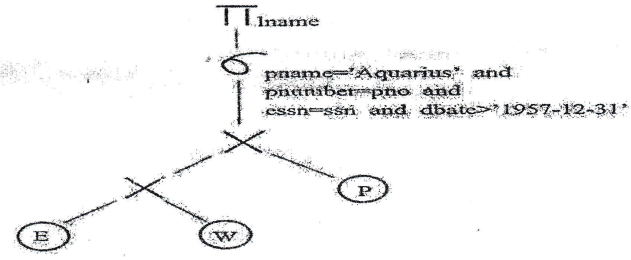
\includegraphics[width=4in]{dbms_1} \hfill [5] (\texttt{81 Ba})\\
            b. 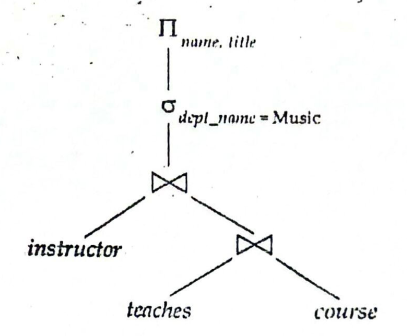
\includegraphics[width=4in]{dbms_2} \hfill [2] (68 Ma)
            
            \item How can you optimize the following query? \hfill [5] (\bo{71 Bh})\\
            $\Pi_{\text{name, title}}\left(\sigma_{\text{dept\_name=``Music"}}(\text{instructor} \bowtie \Pi_{\text{course\_id, title}} (\text{teaches} \bowtie \text{course}))\right)$
        \end{enumerate}
    \subsection{Query Decomposition}
    \subsection{Performance Tuning}

    \pagebreak
\section{File Structure and Hashing}
    \begin{center}(4 Hours/8 Marks)\end{center}
    \subsection{Records Organizations}
		\begin{enumerate}[noitemsep, topsep=0pt]
			\item What is record organization? \hfill [2] (\bo{\texttt{79 Bh}})
			
			\item Explain the way of file organization. \hfill [2] (\bo{\texttt{79 Bh}})
			
			\item Briefly explain Fixed Length Record and Variable Length Record. \hfill [4] (\bo{72 Ash}, 76 Ba, 75 Ba)
			\lb with suitable examples. \hfill [4] (\bo{78 Ch, 75 Bh})
			
			\item Briefly explain how variable length records are stored in databases? \hfill [3] (70 Ma)
			
			\item Discuss the pointer method to represent the variable record by fixed-length representation.
			\enter\hfill [3] (65 Ka)
			
			\item How does anchor and overflow bock improve the pointer method? \hfill [3] (65 Ka)
			
			\item Discuss about sequential file organization and multi-table clustering file organization. \hfill [4] (\bo{74 Bh})
		\end{enumerate}		    
    
    \subsection{Disks and Storage}
    		\begin{enumerate}[noitemsep, topsep=0pt]
    			\item What is RAID? \hfill [1] (\bo{\texttt{81 Bh}, 80 Ch, 77 Ch, 76 Bh, 71 Bh}, \texttt{80 Ba}, 73 Ma) [3] (\bo{68 Bh}, 72 Ma)
    			
			\item What is the use of RAID storage devices? \hfill [2] (\bo{73 Bh}) [3] (\bo{70 Bh})
			
			\item What are the advantages of mirroring? \hfill [2] (\bo{70 Bh})
    			
    			\item Explain different levels of RAID. \hfill [3] (\bo{\texttt{81 Bh}}) [4] (\bo{80 Ch})
    			
			\item Summarize the various levels of RAID and mention how to select an appropriate level of RAID.
			\enter\hfill [3] (\bo{71 Bh}) [3+1] (\bo{79 Ch})
    			
    			\item Explain the types of RAID and mention how to select an appropriate level of RAID.
    			\enter\hfill [3] (\bo{77 Ch, 76 Ch}) [4] (\texttt{80 Ba})
    			
    			\item Which RAID level would you prefer the best for safety of application and why? \hfill [3] (73 Ma)
    			
    			\item Why does RAID Level 6 give better data protection than RAID 5?  \hfill [3] (\bo{78 Ch})
    			
    			\item Briefly explain the RAID level 0 to 6. \hfill [6] (68 Ma)
    		\end{enumerate}
    		
    \subsection{Remote Backup System}
		\begin{enumerate}[noitemsep, topsep=0pt]
			\item Explain about remote back up system. \hfill [3] (\bo{70 Bh})
			\lb with diagram. \hfill [3] (\bo{73 Bh})
		\end{enumerate}		    
    
    \subsection{Hashing Concepts, Static and Dynamic Hashing}
    		\begin{enumerate}[noitemsep, topsep = 0pt]
    			\item What do you mean by hashing? Explain how hashing helps to organize the file with an example.
    			\enter\hfill [4] (\bo{\texttt{81 Bh}})
    			
    			\item Explain about Dynamic hashing techniques in details. \hfill [6] (\texttt{81 Ba})
    			
    			\item Why dynamic hashing is advantageous over static hashing? \hfill [3] (73 Ma)
    			
    			\item Explain the working of static hash indexing along with suitable examples. \hfill [3] (\bo{80 Ch})
    			
    			\item Explain limitation of static hashing? \hfill [2] (\bo{69 Bh})
    			
			\item How extendable hashing overcome limiation of static hashing. \hfill [4] (\bo{69 Bh})
			    			
    			\item What do you mean by hashing and indexing? \hfill [2] (\bo{77 Ch}, 76 Ba)
    		\end{enumerate}
    		
    \subsection{Order Indices}
    		\begin{enumerate}[noitemsep, topsep = 0pt]    			
			\item What is indexing? \hfill [1] (73 Ma)			
    			
    			\item What is the roles of index in DBMS? \hfill [1] (\bo{\texttt{80 Bh}})
    			
    			\item What is secondary index? Explain with example. \hfill [2] (\texttt{81 Ba})
    			
    			\item Explain primary index and secondary index with example. \hfill [4] (\bo{\texttt{80 Bh}})
    			
    			\item What is the difference between ordered indices and hash indices in a database? \hfill [2] (\bo{76 Bh, 71 Bh}, \texttt{80 Ba}, 75 Ba)
			
			\item What do you mean by ordered index and hash index? \hfill [2] (\bo{69 Bh})    			
    			
    			\item What is the advantages of using sparse index? \hfill [2] (\bo{76 Bh, 71 Bh}, 75 Ba) [4] (\texttt{80 Ba})
    			
    			\item Differentiate between dense index and sparse index. \hfill [2] (\bo{79 Ch, 77 Ch}, 76 Ba) [3] (70 Ma) [5] (68 Ma)
    			\lb with examples. \hfill [5] (72 Ma)
    			
    			\item Explain dense index file and sparse index file. \hfill [4] (\bo{74 Bh})
    			
    			\item How is a record searched from a sparse sequential index? \hfill [3] (\bo{73 Bh})
    			
    			\item Explain along with example how a database record is searched using a sparse primary index? \hfill [3] (71 Ma)
    			
    			\item Compare secondary index and multilevel indexing techniques. \hfill [4] (\bo{\texttt{79 Bh}})
    			
    			\item What is index sequential file? \hfill [2] (\bo{79 Ch})
    			
    			\item Write the SQL syntax to create an index. \hfill [1] (71 Ma)
    			\item What is a secondary index. \hfill [2] (70 Ma)
    		\end{enumerate}
    		
    \subsection{B+ tree index}
    		\begin{enumerate}[noitemsep, topsep=0pt]
    			\item What are the characteristics of B\super{+} tree? \hfill [3] (\bo{\texttt{80 Bh}})
    			
    			\item Describe B\super{+} tree structure used for indexing. \hfill [4] (\bo{75 Bh})
    			
    			\item Define B+ tree structure used for indexing. \hfill [4] (\bo{72 Ash})
    			
    			\item Explain the node structure of a B+ tree. \hfill [2] (71 Ma)
    			
    			\item Explain the B+ tree index with an example. \hfill [8] (\bo{68 Bh})
    			
    			\item Why is B+ tree good for indexing? \hfill [2] (71 Ma)
    		\end{enumerate}

    \pagebreak
\section{Transactions processing and Concurrency Control}
    \begin{center}(6 Hours/12 Marks)\end{center}

    \subsection{Transactions}
            \begin{enumerate}[noitemsep, topsep=0pt]
                \item Define transaction. \hfill [1] (\bo{80 Ch, 75 Bh}, 76 Ba, 71 Ma) [2] (72 Ma, \bo{\textit{68 Bh}})
                \lb and its properties. \hfill [3] (\bo{80 Ch})
                \lb and the ideal properties of a transaction. \hfill [4] (77 Ba)

                \item (Assumed) Write short notes on Compensating Transaction. \hfill [4] (65 Ka)

                \item What are the properties a transaction should satisfy in a database system? \hfill [3] (71 Ma)

                \item Explain about the state diagram of transaction. \hfill [3] (\bo{\texttt{80 Bh}, 75 Bh}) [4] (75 Ba)
                \lb During execution, a transaction passes through several states until it finally commits or aborts. Explain all possible sequences of state through which a transaction may pass.
                \enter\hfill [4] (\bo{70 Bh}) [5] (\bo{77 Ch})
                
                \item What are the possible transaction states? \hfill [2] (\bo{76 Bh})

                \item Explain different states of a transaction along with state transition diagram. \hfill [4] (\bo{72 Ash})
            \end{enumerate}

    \subsection{ACID properties}
        \begin{enumerate}[noitemsep, topsep=0pt]
            \item Explain ACID properties in database transaction. \hfill [4] (\bo{74 Bh}, 73 Ma) [5] (\textit{68 Ma})
            \lb with an example. \hfill [4] (\bo{\texttt{81 Bh}, 78 Ch}) [6] (72 Ma) [8] (70 Ma)
            \lb Define transaction and explain its ACID properites. \hfill [1+3] (\bo{\texttt{79 Bh}})

            \item List the ACID properties. Explain the usefulness of each. \hfill [4] (\bo{70 Bh}) [5] (\bo{\textit{67 Mng}})

            \item Explain Atomicity and Isolation properites of a database transaction. \hfill [4] (\bo{71 Bh})

            \item Database-system implementers have paid much more attention to the ACID properites than have file-system implementers. Why might this be the cases? \hfill [4] (\texttt{80 Ba})
        \end{enumerate}

    \subsection{Concurrent Executions}
        \begin{enumerate}
            \item Explain how graph based protocol maintains concurrent execution of transactions. \hfill [4] (\bo{79 Ch})
        \end{enumerate}

    \subsection{Serializability Concept}
        \begin{enumerate}[noitemsep, topsep=0pt]
            \item Define schedule and give proper examples. \hfill [2] (\bo{\texttt{79 Bh}})
            \lb Define schedules. \hfill [2] (\bo{73 Bh})

            \item What is a serializable schedule? \hfill [2] (\bo{\texttt{79 Bh}}) [3] (\bo{\textit{68 Bh}})

            \item What do you mean by serializability of a schedule? \hfill [2] (71 Ma)
            
            \item Explain the concept of conflict serializability. \hfill [4] (\bo{71 Bh}, 73 Ma)
            \lb with an example. \hfill [4] (\bo{72 Ash}, 75 Ba) [8] (\bo{69 Bh})

            \item How to test Conflict Serializability of a Schedule S, explain in details with example. \hfill [5] (\bo{\texttt{80 Bh}})

            \item Describe how conflict serializability differs from the view serializability for concurrent execution of transactions. \hfill [4] (\bo{74 Bh})

            \item Describe the concept of view serializability for concurrent execution of transaction. \hfill [4] (\bo{73 Bh})
            
            \item Check whether the given schedule S is conflict serializable or not. If yes, then determine all the possible serialzed schedules. (\textit{no schedule given lmao}) \hfill [2+6] (\texttt{81 Ba})            

            \item Consider a schedule S: r1(y); r3(z); w1(y); w2(z); r3(y); w2(y). State whether it is conflict serializable schedule or not. Determine the equivalent serial schedule if it is serializable.
            \enter\hfill [4] (\bo{79 Ch})

            \item Which of the following schedule is conflict serializable? For each serializable schedule, determine the equivalent serial schedule. \hfill [4] (\bo{76 Bh})
            \begin{itemize}[noitemsep, topsep=0pt]
                \item r1(X); r3(X); w1(X); r2(X); w3(X)
                \item r1(X); r3(X); w3(X); w1(X); r2(X)
            \end{itemize}
        \end{enumerate}
        
    \subsection{Lock based Protocols}
         \begin{enumerate}[noitemsep, topsep=0pt]
            \item Describe granurality of locking for concurrency control? \hfill [2] (71 Ma)

            \item Differentiate between fine granurality and coarse granularity locking in multiple granularity locking protocol. \hfill [4] (\bo{69 Ch})
            
            \item Explain two phase locking protocol for concurrency control in DBMS. \hfill [4] (\bo{80 Ch, 78 Ch, 72 Ash}, 73 Ma)
            \lb Explain two phase locking protocol with an example. \hfill [4] (\bo{70 Ch}, \texttt{80 Ba})
            \lb Explain two phase locking protocol with its limitations. \hfill [4] (\bo{75 Bh})
            \lb Explain two phase locking protocol briefly. \hfill [2] (\bo{77 Ch}) [3] (76 Ba)

            \item How strict two phase locking protocol improves the two phase locking protocol? \hfill [3] (\textit{65 Ka})

            \item Explain the different types of locks used for concurrency control. Draw the lock compatibility matrix. \hfill [6] (72 Ma)
        \end{enumerate}

    \subsection{Deadlock handling and Prevention}
        \begin{enumerate}[noitemsep, topsep=0pt]
            \item How deadlocks arise in transaction processing? \hfill [2] (\bo{76 Bh, 73 Bh})

            \item Explain wait \& die scheme for deadlock prevention. \hfill [2] (\bo{77 Ch})

            \item Explain the deadlock prevention strategies. \hfill [4] (\bo{73 Bh})
            
            \item Explain how wait-die scheme and wound-wait scheme helps to prevent deadlock. \hfill [4] (\bo{\texttt{81 Bh}})
        \end{enumerate}

    \pagebreak
\section{Crash Recovery}
    \begin{center}(4 Hours/6 Marks)\end{center}
    \subsection{Failure Classification}
    \subsection{Recovery and Atomicity}
    \subsection{Log‐based Recovery}
    \subsection{Shadow paging}
    \subsection{Advanced Recovery Techniques}

    \pagebreak
\section{Advanced database Concepts}
    \begin{center}(4 Hours/6 Marks)\end{center}
    \subsection{Concept of Objet‐Oriented and Distributed Database Model}
    \subsection{Properties of Parallel and Distributed Databases}
    \subsection{Concept of Data warehouse Database}
    \subsection{Concept of Spatial Database}

\end{document}
